\documentclass[a4paper,11pt]{article}
\usepackage{graphicx}
\usepackage{geometry}
\geometry{left=25mm,right=25mm,%
bindingoffset=0mm, top=20mm,bottom=20mm}
\linespread{1.9}
\begin{document}
\begin{table}
\caption{Auto generated table}
\centering
\begin{tabular}{|c|c|c|c|c|}

\hline
(row=0, col=0) & (row=0, col=1) & (row=0, col=2) & (row=0, col=3) & (row=0, col=4) \\
\hline
(row=1, col=0) & (row=1, col=1) & (row=1, col=2) & (row=1, col=3) & (row=1, col=4) \\
\hline
(row=2, col=0) & (row=2, col=1) & (row=2, col=2) & (row=2, col=3) & (row=2, col=4) \\
\hline
(row=3, col=0) & (row=3, col=1) & (row=3, col=2) & (row=3, col=3) & (row=3, col=4) \\
\hline
(row=4, col=0) & (row=4, col=1) & (row=4, col=2) & (row=4, col=3) & (row=4, col=4) \\
\hline

\end{tabular}
\end{table}

\begin{figure}
\caption{Auto generated image}
\centering
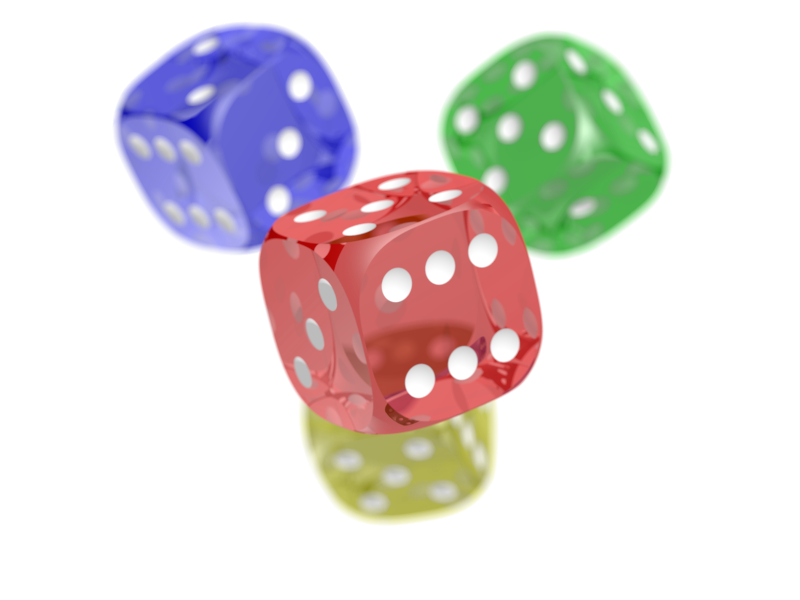
\includegraphics[width=0.5\textwidth]{"../../PNG_transparency_demonstration_1.png"}
\end{figure}

\end{document}
